% !TeX spellcheck = ru_RU
% !TEX root = vkr.tex

\section{Результаты вычислительного эксперимента по определению кода Голланда}

\subsection{Сравнение результатов моделей на полных данных}

Для обеспечения сравнимости различных подходов (регрессия, классификация, ранжирование) между собой основное внимание было уделено мере сходства C-индекс (более подробное описание в подразделе~\ref{subsec:cindex}; чем выше значение, тем лучше; значение для случайного константного предсказателя равно $9.0$). Такой выбор меры позволяет сравнивать результаты с другими научными работами. Так, на основе социо-демографических данных в работе~\cite{Bogacheva} достигается значение $\text{C‑index}~=~10.95$ для регрессии и $\text{C‑index}~=~11.08$ для классификации, поэтому результат предсказания с таким же значением или больше может считаться приемлемым.

\begin{table}[!ht]
  \centering
  \caption{Сравнение регрессионных моделей, C‑индекс}
  \label{tab:regr_res}
    \setlength{\tabcolsep}{2pt}
    \begin{tabular*}{\textwidth}{@{\extracolsep{\fill}} 
      >{\raggedright\arraybackslash}m{6.25cm}  
      | *{4}{>{\centering\arraybackslash}m{2.35cm}}
    @{}}
  \toprule
      \textbf{Модель} 
        & \textbf{Multi\-output}      
        & \textbf{Мult. PCA}   
        & \textbf{Chain}   
        & \textbf{Chain PCA} \\
    \midrule
    Регрессия Lasso (L1)      & \g{11.175} & \g{10.887} & \g{11.175} & \g{11.150} \\
    ExtraTrees                & \g{10.700} & \g{11.100} & \g{10.625} & \g{10.825} \\
    Регрессия Ridge (L2)      & \g{10.988} & \g{10.537} & \g{11.062} & \g{10.412} \\

    \arrayrulecolor[gray]{0.8}
    \specialrule{0.75pt}{0pt}{0pt}
    \arrayrulecolor{black}
    
    Метод опорных векторов    & \g{10.713} & \g{10.950} & \g{10.713} & \g{10.950} \\
    Пошаговая регрессия       & \g{10.605} & \g{10.905} & \g{10.600} & \g{10.905} \\
    CatBoost                  & \g{10.688} & \g{10.812} & \g{10.688} & \g{10.812} \\
    Случайный лес             & \g{10.625} & \g{10.475} & \g{10.812} & \g{10.588} \\
    Линейная регрессия (OLS)  & \g{10.688} & \g{10.800} & \g{10.688} & \g{10.800} \\
    LightGBM                  & \g{10.750} & \g{10.425} & \g{10.750} & \g{10.425} \\
    kNN                       & \g{10.525} & \g{10.400} & \g{10.525} & \g{10.400} \\
    XGBoost                   & \g{9.164}  & \g{9.729}  & \g{9.162}  & \g{9.725}  \\
    Constant baseline         & \g{9.000}  & \g{9.000}  & \g{9.000}  & \g{9.000}  \\
    \midrule
    TabPFN                    & \g{10.562} &            &            &            \\
    MLP (BatchNorm, DropOut, регуляризация) & \g{10.462} &    &            &            \\
    MLP                       & \g{10.275} &            &            &            \\
    \bottomrule
  \end{tabular*}
  \vspace{0.75em}
  \begin{minipage}{\textwidth}
      \small
      \textit{Обозначения:\\
      \hspace*{1em}Mult.~--- multioutput, предсказание переменных независимо друг от друга,\\
      \hspace*{1em}Chain~--- предсказание выходных переменных по цепочке,\\
      \hspace*{1em}PCA~--- метод главных компонент (уменьшение размерности)}
  \end{minipage}
\end{table}

\begingroup
\fontsize{7pt}{8pt}\selectfont
\begin{table}
  \centering
  \caption{Важность признаков модели случайного леса}
  \label{tab:feature_imp}
  \begin{tabular*}{\textwidth}{@{\extracolsep{\fill}} 
      >{\centering\arraybackslash}p{2.25cm}|
      >{\raggedright\arraybackslash}p{9cm}|c c @{}}
    \toprule
    \makecell{Код\\признака} 
      & \makecell[c]{Наименование признака} 
      & \makecell{Важность\\(\%)} 
      & \makecell{Накоплено\\(\%)} \\
    \midrule
    CT\_1   & Открытость--замкнутость                & 15.5 & 15.5 \\
    CT\_7   & Чувственность--твердость               & 15.5 & 31.0 \\
    SC\_19  & Гедонизм--индивидуальный приоритет     & 4.2  & 35.2 \\
    EY\_1   & Экстраверсия                           & 4.0  & 39.2 \\
    CT\_4   & Беспечность--озабоченность             & 3.6  & 42.8 \\
    SC\_3   & Власть--нормативный идеал              & 3.4  & 46.2 \\
    LN\_3   & Циклотимность                          & 3.3  & 49.5 \\
    BF\_3   & Самоконтроль--импульсивность           & 2.5  & 52.0 \\
    BF\_4   & Эмоц. устойчивость--неустойчивость     & 2.5  & 54.5 \\
    \bottomrule
  \end{tabular*}
\end{table}
\endgroup


Результаты определения кода Голланда как задачи регрессии (на основе C-индекса) приведены в таблице~\ref{tab:regr_res}. В сравнении с константным предсказателем модель XGBoost показывает низкие результаты. Наилучшие результаты показывает регуляризованная регрессия (Lasso и Ridge): $\text{C‑index}~=~11.175$ и $\text{C‑index}~=~11.062$. Высокий результат показывает модель ExtraTrees: $\text{C‑index}~=~11.1$. Лучшая из нейросетевых моделей, foundation-модель TabPFN, $\text{C‑index}~=~10.562$, показывает результат лучше лишь XGBoost и на одном уровне с методом k-ближайших соседей. Стоит отметить, что результаты моделей при различных подходах, независимом и по цепочке (\emph{multioutput} и \emph{chain}), практически идентичны. В то же время попарно для каждого из подходов лучшие результаты многие модели показывают на наборе данных меньшей размерности (после применения метода главных компонент, PCA), кроме регуляризованных линейных регрессий. 

% Сравнение регрессионных моделей по метрике RMSE приведено в таблице~\ref{tab:regr_res_rmse}.
% \newcommand{\grmse}[1]{\gradientcelld{#1}{2.0}{2.1}{2.8}{high}{mid}{low}{70}}

\begingroup
    \fontsize{8pt}{9pt}\selectfont
    \begin{table}
      \centering
      \caption{Сравнение регрессионных моделей, метрика RMSE}
      \label{tab:regr_res_rmse}
        \setlength{\tabcolsep}{2pt}
        \begin{tabular*}{\textwidth}{@{\extracolsep{\fill}} 
          >{\raggedright\arraybackslash}m{6.25cm}  
          | *{4}{>{\centering\arraybackslash}m{2.35cm}}
        @{}}
      \toprule
          \textbf{Модель} 
            & \textbf{Multi\-output}      
            & \textbf{Мult. PCA}    
            & \textbf{Chain}   
            & \textbf{Chain PCA} \\
        \midrule
        Регрессия Lasso (L1)      & \grmse{2.018} & \grmse{2.036} & \grmse{2.018} & \grmse{2.030} \\
        Линейная регрессия (OLS)  & \grmse{2.155} & \grmse{2.019} & \grmse{2.155} & \grmse{2.019} \\
        Регрессия Ridge (L2)      & \grmse{2.025} & \grmse{2.037} & \grmse{2.028} & \grmse{2.044} \\
        Пошаговая регрессия       & \grmse{2.094} & \grmse{2.027} & \grmse{2.094} & \grmse{2.027} \\
        CatBoost                  & \grmse{2.044} & \grmse{2.096} & \grmse{2.044} & \grmse{2.096} \\
        Случайный лес             & \grmse{2.069} & \grmse{2.131} & \grmse{2.070} & \grmse{2.133} \\
        LightGBM                  & \grmse{2.074} & \grmse{2.128} & \grmse{2.074} & \grmse{2.128} \\
        Метод опорных векторов    & \grmse{2.100} & \grmse{2.101} & \grmse{2.100} & \grmse{2.101} \\
        ExtraTrees                & \grmse{2.100} & \grmse{2.150} & \grmse{2.112} & \grmse{2.152} \\
        kNN                       & \grmse{2.162} & \grmse{2.151} & \grmse{2.162} & \grmse{2.151} \\
        Constant baseline         & \grmse{2.308} & \grmse{2.308} & \grmse{2.308} & \grmse{2.308} \\
        XGBoost                   & \grmse{2.317} & \grmse{2.314} & \grmse{2.317} & \grmse{2.314} \\
        \midrule
        TabPFN                    & \grmse{2.056} &            &            &            \\
        MLP (BatchNorm, DropOut, регул-я) & \grmse{2.143} &            &            &            \\
        MLP                       & \grmse{2.442} &            &            &            \\
        \bottomrule
      \end{tabular*}
      \vspace{0.75em}
      \begin{minipage}{\textwidth}
          \small
          \textit{Обозначения:\\
          \hspace*{1em}Mult.~--- multioutput, предсказание переменных независимо друг от друга,\\
          \hspace*{1em}Chain~--- предсказание выходных переменных по цепочке,\\
          \hspace*{1em}PCA~--- метод главных компонент (уменьшение размерности)}
      \end{minipage}
    \end{table}
\endgroup

\renewcommand{\g}[1]{\gradientcelld{#1}{9}{11.1}{11.8}{low}{mid}{high}{70}}

\begingroup
  \scriptsize
  \begin{table}
    \centering
    \caption{Сравнение методов подбора весов ансамбля регрессионных моделей}
    \label{tab:regr_ensembles}
    \begin{tabular*}{\textwidth}{@{\extracolsep{\fill}}
        >{\raggedright\arraybackslash}m{8cm}|
        *{4}{>{\centering\arraybackslash}m{1.77cm}}
      @{}}
      \toprule
        \multicolumn{1}{>{\centering\arraybackslash}m{8cm}|}{\textbf{Метод подбора весов}} 
          & \textbf{Multi\-output} 
          & \textbf{Mult. топ-5} 
          & \textbf{Chain} 
          & \textbf{Chain топ-5} \\
      \midrule
      Равные веса всех моделей       & \g{11.063} & \g{11.088} & \g{11.050} & \g{11.013} \\
      Вектор Шэпли (Shap)            & \g{11.050} & \g{11.138} & \g{11.138} & \g{11.050} \\
      Частичный перебор по сетке     & \g{11.550} & \g{11.388} & \g{11.538} & \g{11.325} \\
      Квадратичная оптимизация (QP)  & \g{10.588} & \g{10.463} & \g{10.738} & \g{10.813} \\
      Генетический алгоритм (GA)     & \g{11.500} & \g{11.550} & \g{11.300} & \g{11.563} \\
      Метод роя частиц (PSO)         & \g{11.600} & \g{11.663} & \g{11.613} & \g{11.613} \\
      Координатный спуск             & \g{11.188} & \g{11.225} & \g{11.288} & \g{11.413} \\
      \midrule
      Линейные регрессии с регуляризацией 
        & \multicolumn{2}{c}{Линейная регр.} 
        & \multicolumn{2}{c}{\g{10.887}} \\
      Lasso, Ridge, LightGBM, CatBoost, RF 
        & \multicolumn{2}{c}{Линейная регр.} 
        & \multicolumn{2}{c}{\g{10.688}} \\
      \bottomrule
    \end{tabular*}
    \vspace{0.5em}
    \begin{minipage}{\textwidth}
      \small
      \textit{Обозначения:\\
      \hspace*{1em}Mult.~--- Multioutput, топ-5~--- подбор весов только для топ-5 моделей по C-индексу}
    \end{minipage}
  \end{table}
\endgroup


На примере модели случайного леса (\emph{Random Forest}) в таблице~\ref{tab:feature_imp} приведен анализ важности признаков. Так, два фактора из модели Кеттелла покрывают более 30\% важности всех 55 факторов, 8 факторов~--- более 50\%. В Random Forest важность признака (\emph{gain})~--- это усреднённая по всем деревьям сумма уменьшений критерия нечистоты (Джини или энтропии) на узлах, где при разбиении использовался этот признак. При аналогичном анализе важности признаков с помощью моделей градиентного бустинга получаются схожие результаты: наиболее важными признаются схожие признаки, но они имеют меньшую важность.

\begin{table}[bht]
    \setlength{\tabcolsep}{0pt}
    \centering
    \caption{Весовые коэффициенты моделей и C-индекс для PSO}
    \label{tab:pso_regr_weights}
    \begin{tabular*}{\textwidth}{@{\extracolsep{\fill}} 
        l*{4}{c}>{\centering\arraybackslash}p{1.3cm}
        >{\raggedright\arraybackslash}p{1.3cm}@{}}
        \toprule
        \textbf{Подбор} & \multicolumn{4}{c}{\textbf{Веса моделей}} & \textbf{\quad C-} \\
        \cmidrule(lr){2-5}
        \textbf{весов} & Lasso L1 & Пошаговая регр. & CatBoost & ExtraTrees & \textbf{индекс} \\
        \midrule
        PSO & 0.432 & 0.327 & 0.150 & 0.091 & 11.663 \\
        \bottomrule
    \end{tabular*}
\end{table}


Сравнение методов подбора весов ансамбля регрессионных моделей представлено в таблице~\ref{tab:regr_ensembles}. Лучшим методом подбора весов для моделей линейного блендинга (взвешенного ансамблирования) является метод роя частиц (PSO), $\text{C‑index}~=~11.663$. В таблице~\ref{tab:pso_regr_weights} приведены веса входящих в лучшую PSO-модель базовых регрессоров: наибольший вклад вносит Lasso-регрессор (43.2\%), а также пошаговая регрессия. Модели стекинга показывают результаты хуже, чем модели линейного блендинга.

% Удалим глобальную настройку tabcolsep
% \setlength{\tabcolsep}{6pt}  % удалено

\begin{table}
  \centering
  \caption{Сравнение подходов к классификации (Top-K accuracy)}
  \label{tab:classif_res}
  {\setlength{\tabcolsep}{8pt}
  \begin{tabular*}{\textwidth}{@{\extracolsep{\fill}} 
    p{3.8cm}|
    *{3}{>{\centering\arraybackslash}p{0.83cm}}|
    *{3}{>{\centering\arraybackslash}p{0.83cm}}|
    *{3}{>{\centering\arraybackslash}p{0.83cm}}
  @{}  }
    \toprule
    \multicolumn{1}{@{}p{3.8cm}@{}}{\centering\textbf{Модель}}  
      & \multicolumn{3}{|c|}{\textbf{Multiclass}}
      & \multicolumn{3}{c|}{\textbf{Multilabel}}
      & \multicolumn{3}{c}{\textbf{Label Powerset}} \\
    \cmidrule(lr){2-4}\cmidrule(lr){5-7}\cmidrule(lr){8-10}
      & Top1 & Top2 & Top3 
      & Top1 & Top2 & Top3 
      & Top1 & Top2 & Top3 \\
    \midrule
    kNN             & 0.99 & 0.71 & 0.13 & 1.00 & 0.76 & 0.11 & 0.98 & 0.65 & 0.18 \\
    Логист. L1-регр.& 1.00 & 0.70 & 0.16 & 1.00 & 0.70 & 0.16 & 0.99 & 0.64 & 0.10 \\
    XGBoost         & 1.00 & 0.70 & 0.11 & 0.98 & 0.68 & 0.10 & 0.96 & 0.63 & 0.11 \\
    Логист. L2-регр.& 1.00 & 0.70 & 0.15 & 0.99 & 0.70 & 0.21 & 0.99 & 0.68 & 0.09 \\
    Наивный Байес   & 0.98 & 0.70 & 0.15 & 0.99 & 0.70 & 0.15 & 0.99 & 0.69 & 0.16 \\
    ExtraTrees      & 1.00 & 0.73 & 0.15 & 1.00 & 0.78 & 0.15 & 0.98 & 0.69 & 0.20 \\
    SVM             & 1.00 & 0.74 & 0.15 & 1.00 & 0.72 & 0.14 & 0.98 & 0.68 & 0.21 \\
    Random Forest   & 1.00 & 0.74 & 0.16 & 1.00 & 0.74 & 0.15 & 0.99 & 0.64 & 0.23 \\
    CatBoost        & 0.99 & 0.79 & 0.11 & 0.99 & 0.79 & 0.11 & 0.99 & 0.70 & 0.16 \\
    LightGBM        & 0.98 & 0.56 & 0.05 & 0.98 & 0.70 & 0.10 & 0.95 & 0.53 & 0.05 \\
    \bottomrule
  \end{tabular*}}
\end{table}


На рисунке~\ref{fig:cindex_distr} показана гистограмма распределения значений C-индекса для предсказаний PSO-ансамбля регрессоров. Заметно, что распределение \enquote{скошено} влево относительно медианы; большая часть значений лежит правее константного значения $\text{C‑index}~=~9.0$.

\renewcommand{\g}[1]{\gradientcelld{#1}{7}{10.35}{11.3}{low}{mid}{high}{70}}
  
\begingroup
\fontsize{8pt}{9pt}\selectfont
\setlength{\tabcolsep}{0pt}
\begin{table}[hbt!]
  \centering
  \caption{Сравнение классификаторов}
  \label{tab:best_classif}
  \begin{tabular*}{\textwidth}{@{\extracolsep{\fill}}
    >{\raggedright\arraybackslash}p{4cm}      % Классификатор
    >{\centering\arraybackslash}p{2cm}          % Подход
    >{\centering\arraybackslash}p{2.6cm}        % C‑индекс
    *{3}{>{\centering\arraybackslash}p{1.1cm}}  % Top‑1,2,3
  @{}}
    \toprule
    \textbf{Классификатор}
      & \textbf{Подход}
      & \textbf{C‑индекс}
      & \textbf{Top1}
      & \textbf{Top2}
      & \textbf{Top3} \\
    \midrule
    kNN                  & Multilabel & \g{10.838} & 1.000 & 0.763 & 0.113 \\
    Логист. L1-регр.     & Multiclass & \g{10.663} & 1.000 & 0.700 & 0.163 \\
    XGBoost              & Multiclass & \g{10.638} & 1.000 & 0.700 & 0.113 \\
    Логист. L2-регр.     & Multiclass & \g{10.500} & 1.000 & 0.700 & 0.150 \\
    Наивный Байес        & Multilabel & \g{10.350} & 0.988 & 0.700 & 0.150 \\
    ExtraTrees           & Multilabel & \g{10.013} & 1.000 & 0.775 & 0.146 \\
    SVM                  & Multilabel & \g{9.875}  & 1.000 & 0.721 & 0.138 \\
    Random Forest        & Multilabel & \g{9.800}  & 0.996 & 0.738 & 0.146 \\
    CatBoost             & Multilabel & \g{9.775}  & 0.988 & 0.788 & 0.113 \\
    LightGBM             & Multilabel & \g{9.313}  & 0.975 & 0.700 & 0.100 \\
    Baseline (случ.) & –          & \g{9.000}  & 0.950 & 0.500 & 0.050 \\
    \bottomrule
  \end{tabular*}
\end{table}
\endgroup

\begin{figure}[htbp]
    \centering
    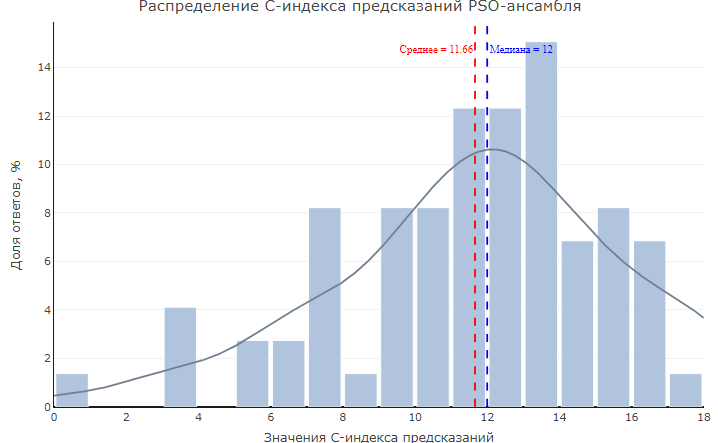
\includegraphics[width=0.95\linewidth]{figures/Cindex_distr_PSO_regr.png}
    \caption{Распределение значений C-индекса для предсказаний PSO-ансамбля регрессоров}
    \label{fig:cindex_distr}
\end{figure}

Сравнение моделей базовых классификаторов в разрезе трех главных подходов для классификации показано в таблице~\ref{tab:classif_res}. Сравнение производилось по метрике Top-K точность. Подходы \emph{multiclass} и \emph{multilabel} показывают схожие результаты и опережают подход \emph{label powerset} по метрикам точности Top-1 и Top-2. Можно заметить, что большинство моделей в 98--100\% случаев верно предсказывают в тройке кодов хотя бы один код, который действительно есть в фактических данных в \emph{верхней триаде}; в 70\% и более угадываются хотя бы два кода. Лишь примерно в 15\% правильно предсказываются все три кода одновременно. 

\renewcommand{\g}[1]{\gradientcelld{#1}{8}{10.8}{11.7}{low}{mid}{high}{70}}

\begingroup
    \fontsize{8pt}{9pt}\selectfont
    \setlength{\tabcolsep}{0pt}
    \begin{table}
      \centering
      \caption{Сравнение методов подбора весов ансамбля классификаторов}
      \label{tab:clsf_ensemble}
      \begin{tabular*}{\textwidth}{@{\extracolsep{\fill}}
        >{\raggedright\arraybackslash}m{8cm} 
        *{3}{>{\centering\arraybackslash}m{2.75cm}} @{}}
        \toprule
        \textbf{Метод подбора весов}
          & \textbf{Multiclass}
          & \textbf{Multilabel}
          & \textbf{Label Powerset} \\
        \midrule
        Равные веса всех моделей      & \g{10.663} & \g{10.888} & \g{10.563} \\
        Вектор Шэпли (Shap)           & \g{10.563} & \g{11.038} & \g{10.525} \\
        Частичный перебор по сетке    & \g{11.213} & \g{11.488} & \g{11.525} \\
        Квадратичная оптимизация (QP) & \g{10.488} & \g{10.638} & \g{10.650} \\
        Генетический алгоритм (GA)    & \g{11.263} & \g{11.313} & \g{11.213} \\
        Метод роя частиц (PSO)        & \g{11.263} & \g{11.625} & \g{11.525} \\
        Координатный спуск            & \g{11.200} & \g{11.275} & \g{10.425} \\
        \bottomrule
      \end{tabular*}
    \end{table}
\endgroup


В таблице~\ref{tab:best_classif} приведено сравнение лучших базовых моделей классификации. На первом месте с $\text{C‑index}~=~10.838$ метод k-ближайших соседей (подход \emph{multilabel}), за ним логистическая Lasso-регрессия (\emph{multiclass}) с $\text{C‑index}~=~10.663$.

\begin{table}
    \setlength{\tabcolsep}{0pt}
    \centering
    \caption{Весовые коэффициенты моделей и C‑индекс для PSO}
    \label{tab:clsf_pso_w}
    \begin{tabular*}{\textwidth}{@{\extracolsep{\fill}} 
          >{\centering\arraybackslash}p{1.5cm}
          *{5}{c}>{\centering\arraybackslash}p{1.3cm}
          >{\raggedright\arraybackslash}p{1.2cm}
        @{}}
          \toprule
          \textbf{Подбор} & \multicolumn{5}{c}{\textbf{Веса моделей}} & \textbf{\quad C-}\\
          \cmidrule(lr){2-6}
          \textbf{весов} & kNN & SVM & Logit L1 & XGBoost & LightGBM & \textbf{индекс}\\
          \midrule
          PSO & 0.291 & 0.164 & 0.191 & 0.183 & 0.151 & 11.625 \\
          \bottomrule
    \end{tabular*}
\end{table}


Сравнение методов подбора весов ансамбля классификаторов представлено в таблице~\ref{tab:clsf_ensemble}. Лучшим методом подбора весов для моделей линейного блендинга (взвешенного ансамблирования) является метод роя частиц (PSO), $\text{C‑index}~=~11.625$. В таблице~\ref{tab:clsf_pso_w} приведены веса классификаторов, которые определены с помощью PSO: наибольший вклад вносят kNN и L1-регрессия. Таким образом, результаты лучшего взвешенного ансамбля классификаторов лишь немного хуже лучшего регрессионного ансамбля.

\renewcommand{\g}[1]{\gradientcelld{#1}{7}{9.6}{11.5}{low}{mid}{high}{70}}
\newcommand{\gndcg}[1]{\gradientcelld{#1}{0.25}{0.54}{0.7}{low}{mid}{high}{70}}

\begingroup
    \setlength{\tabcolsep}{0pt}
    \begin{table}
        \fontsize{14pt}{14pt}\selectfont
        \centering
        \caption{Сравнение моделей ранжирования}
        \label{tab:rank}
        \begin{tabular*}{\textwidth}{@{\extracolsep{\fill}} 
          >{\raggedright\arraybackslash}p{3cm}  % Функция потерь
          | *{3}{>{\centering\arraybackslash}p{2.2cm}}  % C‑индекс
          | *{3}{>{\centering\arraybackslash}p{2.2cm}}  % NDCG@3
        }
          \toprule
            \multicolumn{1}{c|}{\textbf{Функция}}  
              & \multicolumn{3}{c|}{\textbf{C‑индекс}} 
              & \multicolumn{3}{c}{\textbf{NDCG@3}} \\
            \cmidrule(lr){2-4} \cmidrule(lr){5-7}
            \multicolumn{1}{c|}{\textbf{потерь}}  
            & Deep \& Cross 
            & Trans\-former 
            & MLP 
            & Deep \& Cross 
            & Trans\-former 
            & MLP \\
          \midrule
          ApproxNDCG   & \g{10.025} & \g{8.888}  & \g{9.150}  & \gndcg{0.539} & \gndcg{0.439} & \gndcg{0.388} \\
          LambdaRank   & \g{9.963}  & \g{9.675}  & \g{9.650}  & \gndcg{0.527} & \gndcg{0.489} & \gndcg{0.543} \\
          ListNet@1    & \g{9.650}  & \g{10.325} & \g{10.438} & \gndcg{0.504} & \gndcg{0.628} & \gndcg{0.653} \\
          ListNet@3    & \g{9.450}  & \g{9.950}  & \g{10.788} & \gndcg{0.458} & \gndcg{0.622} & \gndcg{0.638} \\
          \bottomrule
        \end{tabular*}
    \end{table}
\endgroup


Сравнение моделей ранжирования отражено в таблице~\ref{tab:rank}. Лучшая из моделей, многослойный перцептрон с функцией потерь ListNet@3, показывает $\text{C‑index}~=~10.788$, что заведомо хуже, чем лучшие из базовых регрессоров и классификаторов.

\renewcommand{\g}[1]{\gradientcelld{#1}{10}{10.65}{11.7}{low}{mid}{high}{60}}

\begin{table}[!b]
    \fontsize{14pt}{18pt}\selectfont
    \setlength{\tabcolsep}{0pt}
    \centering
    \caption{Обзор лучших моделей для каждого типа задач}
    \label{tab:summary}
    \begin{tabular*}{\textwidth}{@{\extracolsep{\fill}}
        >{\raggedright\arraybackslash}m{4.0cm}   % Тип задач
        | >{\raggedright\arraybackslash}m{3.7cm} % Подход
        | >{\raggedright\arraybackslash}m{5.9cm}   % Лучшая модель
        | >{\centering\arraybackslash}m{2.65cm}     % C‑индекс
        @{}}
        \toprule
        \multicolumn{1}{c|}{\textbf{Тип задач}}
          & \multicolumn{1}{c|}{\textbf{Подход}}
          & \multicolumn{1}{c|}{\textbf{Лучшая модель}}
          & \multicolumn{1}{c}{\textbf{C-индекс}} \\
        \specialrule{0.2pt}{1pt}{1pt}
        Регрессия       & Блендинг, mo
                        & PSO (L1-регрессия, пошаговая регрессия, CatBoost, ExtraTrees)
                        & \g{11.663} \\
        \specialrule{0.2pt}{1pt}{1pt}
        Классификация   & Блендинг, ml
                        & PSO (kNN, SVM, логистич. L1-регр., XGBoost, LightGBM и др.)
                        & \g{11.625} \\
        \specialrule{0.2pt}{1pt}{1pt}
        Регрессия       & Блендинг, chain
                        & PSO
                        & \g{11.613} \\
        \specialrule{0.2pt}{1pt}{1pt}
        Классификация   & Блендинг, lp
                        & PSO / поиск по сетке
                        & \g{11.525} \\
        \specialrule{0.2pt}{1pt}{1pt}
        Классификация   & Блендинг, mc
                        & Генетический алг. / PSO
                        & \g{11.263} \\
        \specialrule{0.2pt}{1pt}{1pt}
        Регрессия       & Multioutput
                        & L1-регрессия
                        & \g{11.175} \\
        \specialrule{0.2pt}{1pt}{1pt}
        Регрессия       & Chain
                        & L2-регрессия
                        & \g{11.062} \\
        \specialrule{0.2pt}{1pt}{1pt}
        Классификация   & Multilabel
                        & kNN
                        & \g{10.838} \\
        \specialrule{0.2pt}{1pt}{1pt}
        Ранжирование    & Списочное
                        & MLP с ListNet@3
                        & \g{10.788} \\
        \specialrule{0.2pt}{1pt}{1pt}
        Классификация   & Multiclass
                        & Логистич. L1-регрессия
                        & \g{10.663} \\
        \bottomrule
    \end{tabular*}
    \begin{minipage}{\textwidth}
      \small
      \textit{Обозначения:\\
      \hspace*{1em}mo~--- Multioutput, ml~--- Multilabel, lp~--- Label Powerset, mc~--- Multiclass,\\
      \hspace*{1em}MLP~--- многослойный перцептрон, PSO~--- метод роя частиц,\\
      \hspace*{1em}SVM~--- метод опорных векторов, kNN~--- метод k-ближайших соседей}
    \end{minipage}
\end{table}

Лучшие из моделей по каждому рассматриваемому типу задач приведены в таблице~\ref{tab:summary}. Двумя лучшими моделями оказались линейные блендинги, веса которых подобраны методом роя частиц: это подходы \emph{multioutput} для регрессии ($\text{C‑index}~=~11.663$) и \emph{multilabel} для классификации ($\text{C‑index}~=~11.625$). Результаты базовых моделей уступают результатам их комбинаций в виде взвешенных ансамблей. 

\subsection{Сравнение подходов к восстановлению данных тестов}

\renewcommand{\g}[1]{\gradientcelld{#1}{7}{9.6}{10.9}{low}{mid}{high}{70}}
  
  \begingroup
    \fontsize{8pt}{9pt}\selectfont
    \setlength{\tabcolsep}{3pt}
    \begin{table}[!b]
      \centering
      \caption{Восстановление значений незаполненных психометрических тестов}
      \label{tab:impute}
      \begin{tabular*}{\textwidth}{@{\extracolsep{\fill}} 
        >{\raggedright\arraybackslash}m{6cm} 
        *{4}{>{\centering\arraybackslash}m{2.4cm}}
      @{}}
        \toprule
        \textbf{Модель-регрессор}
          & \textbf{MICE}
          & \textbf{Soft Impute}
          & \textbf{Маски}
          & \textbf{Ансам\-бли} \\
        \midrule
        Регрессия Lasso (L1)   & \g{9.191} & \g{10.248}  & \g{9.998} & \g{9.866} \\
        Пошаговая регрессия    & \g{9.608} & \g{10.183}  & \g{9.978} & \g{10.082}\\
        Random Forest          & \g{9.518} & \g{10.136}  & \g{9.819} & \g{9.712} \\
        LightGBM               & \g{9.372} & \g{10.086}  & \g{9.686} & \g{9.594} \\
        Линейная регр. (OLS)   & \g{9.407} & \g{10.021}  & \g{9.876} & \g{10.012}\\
        Регрессия Ridge (L2)   & \g{9.442} & \g{9.770}   & \g{9.868} & \g{9.933} \\
        ExtraTrees             & \g{9.101} & \g{9.823}   & \g{9.870} & \g{9.808} \\
        Метод опорных векторов & \g{9.221} & \g{9.814}   & \g{9.864} & \g{9.760} \\
        CatBoost               & \g{9.131} & \g{9.814}   & \g{9.835} & \g{9.461} \\
        kNN                    & \g{9.372} & \g{9.834}   & \g{9.830} & \g{9.377} \\
        XGBoost                & \g{8.769} & \g{9.571}   & \g{9.267} & \g{9.614} \\
        Constant baseline      & \g{9.000} & \g{9.000}   & \g{9.000} & \g{9.000} \\
        \bottomrule
      \end{tabular*}
    \end{table}
  \endgroup

Результаты предсказания регрессионных моделей с использованием различных подходов к восстановлению значений незаполненных психометрических тестов представлены в таблице~\ref{tab:impute}. Лучшие базовые модели для восстановления результатов~--- это Lasso- и пошаговый регрессоры в сочетании с подходом мягкого матричного восстановления данных ($\text{C‑index}~=~10.248$ и $\text{C‑index}~=~10.183$). Ансамблирование моделей, обученных на данных заполненных тестов по отдельности, затем объединенных воедино в зависимости от наличия того или иного теста, показывает следующие результаты: наибольшее значение С-индекса для пошаговой моделей регрессии лишь немного хуже подхода \emph{Soft Impute}: $\text{C‑index}~=~10.082$, однако ансамблевый подход по отдельным тестам требует обучения для всех 31 комбинации наличия тестов. Применение масочного подхода к восстановлению данных в меньшей степени зависит от выбора базовой модели. Хуже всего себя показывает подход множественной импутации (\emph{MICE}).
\renewcommand{\g}[1]{\gradientcelld{#1}{9}{10.25}{11}{low}{mid}{high}{70}}

\begin{table}
  \setlength{\tabcolsep}{0pt}
  \centering
  \caption{Весовые коэффициенты моделей и C-индекс при разных методах подбора весов для ансамблей на восстановленных данных}
  \label{tab:impute_ens}
  \begin{tabular*}{\textwidth}{@{\extracolsep{\fill}} 
        >{\raggedright\arraybackslash}m{1.5cm}
        *{5}{c}
        >{\centering\arraybackslash}m{1.9cm}
      @{}}
    \toprule
    \textbf{Подбор} 
      & \multicolumn{5}{c}{\textbf{Веса моделей}} 
      & \textbf{C-}\\
    \cmidrule(lr){2-6}
    \textbf{весов} 
      & \textbf{Lasso L1} 
      & \textbf{Пошаг.} 
      & \textbf{LightGBM} 
      & \textbf{Случ. лес} 
      & \textbf{kNN} 
      & \textbf{индекс} \\
    \midrule
    PSO    & 0.001 & 0.481 & 0.038 & 0.475 & 0.005 & \g{10.740} \\
    Grid   & 0.000 & 0.500 & 0.000 & 0.500 & 0.000 & \g{10.657} \\
    GA     & 0.281 & 0.369 & 0.109 & 0.189 & 0.052 & \g{10.401} \\
    Спуск  & 0.019 & 0.422 & 0.067 & 0.305 & 0.187 & \g{10.245} \\
    QP     & 0.050 & 0.000 & 0.390 & 0.007 & 0.553 & \g{10.065} \\
    Равные & 0.200 & 0.200 & 0.200 & 0.200 & 0.200 & \g{10.053} \\
    Шэпли  & 0.247 & 0.185 & 0.206 & 0.179 & 0.183 & \g{10.047} \\
    \bottomrule
  \end{tabular*}
  \vspace{0.5em}
  \begin{minipage}{\textwidth}
    \small
    \textit{Обозначения:\\
    \hspace*{1em}PSO~--- метод роя частиц, Grid~--- частичный перебор по сетке,\\
    \hspace*{1em}GA~--- генетический алгоритм, спуск~--- координатный спуск,\\
    \hspace*{1em}QP~--- квадратичная оптимизация, пошаг. ~--- пошаговая регрессия,\\
    \hspace*{1em}случ. лес~--- случайный лес (Random Forest), kNN~--- метод k-ближайших соседей}
  \end{minipage}
\end{table}



В таблице~\ref{tab:impute_ens} был применен лучший из подходов к восстановлению данных, мягкое матричное восстановление, и проведен вычислительный эксперимент с регрессионными моделями, как если бы данные были полными. Для ансамблирования были взяты топ-5 моделей, показавших наибольшие значения меры сходства на этих данных по отдельности. Наилучший результат достигнут при подборе весов для ансамбля с помощью метода роя частиц (\emph{PSO}): $\text{C‑index}~=~10.74$, где наибольший вклад вносят модели пошаговой регрессии (48.1\%) и случайного леса (47.5\%). Таким образом, ансамблирование позволяет значительно улучшить результаты предсказания на восстановленных данных, однако значения меры сходства на восстановленных данных ниже, чем на полных данных для аналогичных моделей регрессии и классификации.